\subsection{System response}
    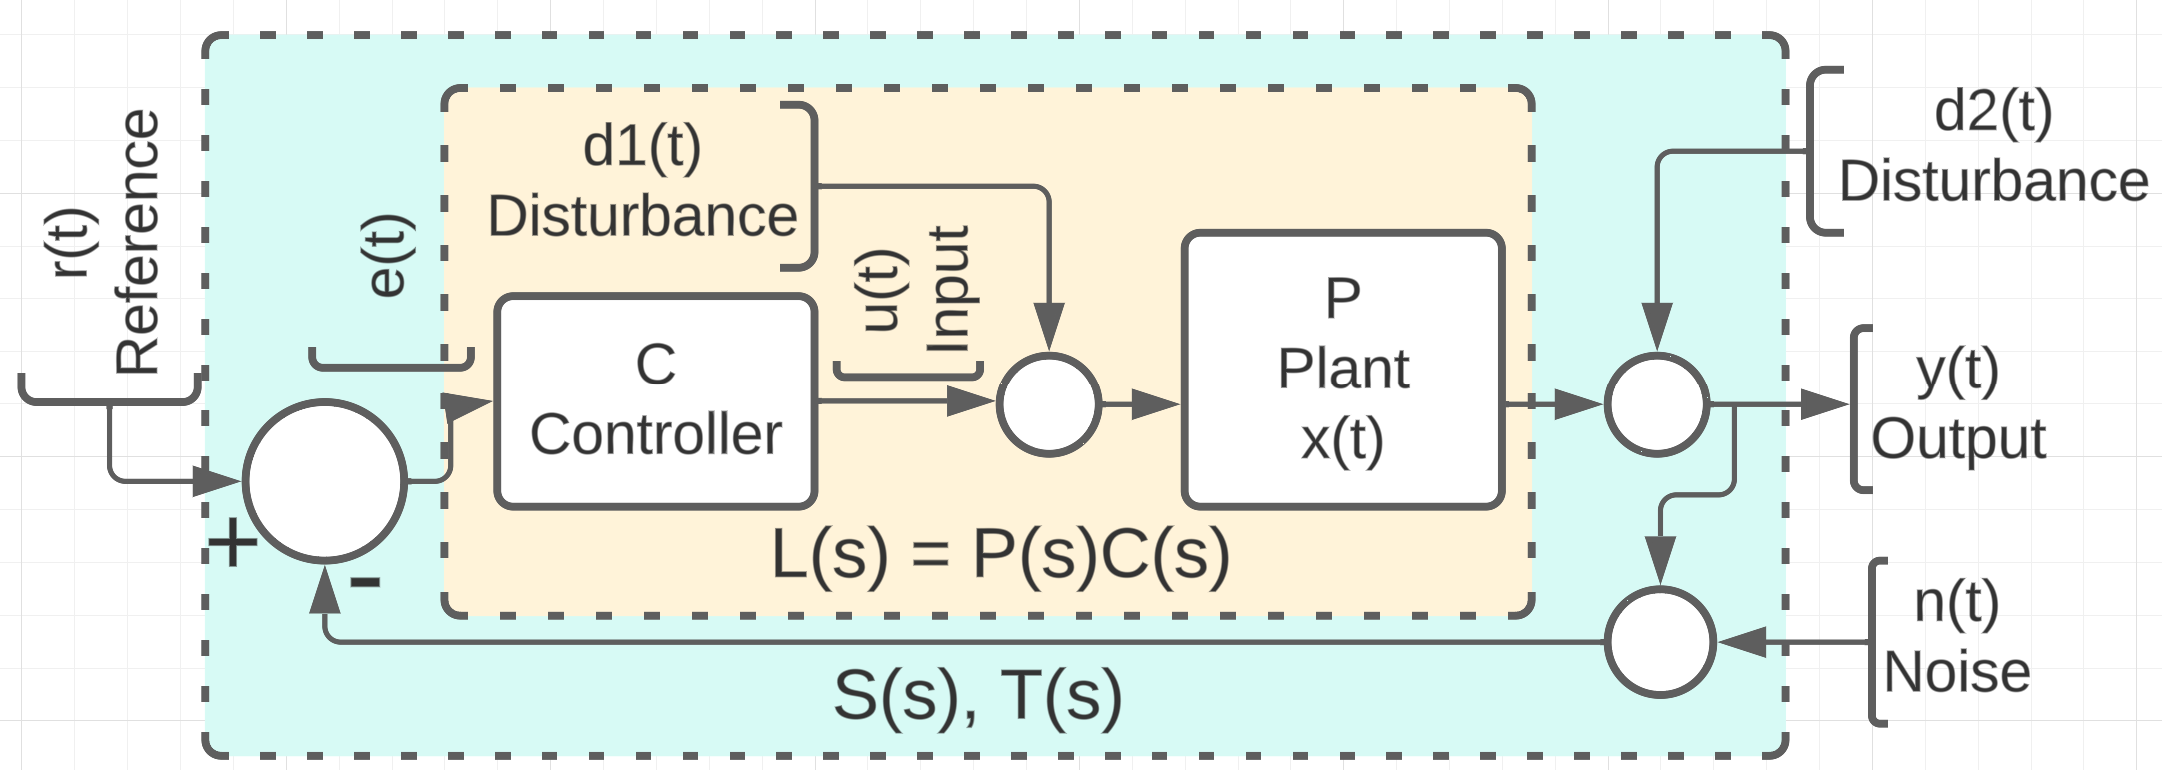
\includegraphics[width = \linewidth]{src/images/basic_block_chart.png}
    \begin{minipage}{0.33\linewidth}
        \titel{Sensitivity}
        \begin{center}
            $S(s) = \frac{1}{1 + L(s)}$
        \end{center}
    \end{minipage}
    \begin{minipage}{0.33\linewidth}
        \titel{Complimentary Sensitivity}
        \begin{center}
            $T(s) = \frac{L(s)}{1 + L(s)}$
        \end{center}
    \end{minipage}
    \begin{minipage}{0.31\linewidth}
        \hfill \break \hfill \break
        $S(s) + T(s) = 1$
    \end{minipage}
    In Nyquist plot of $T(s)$: $|S(s)| = $ Distance to $- \frac{1}{k}$
    
    \subsubsection{steady state error, disturbance and noise}
    find steady state using final value theorem $\lim\limits_{t \rightarrow \infty} a(t) = \lim\limits_{s \rightarrow 0} A(s)$

    \begin{tabular}{|l||*{3}{c|}}\hline
        \backslashbox{From}{To}     &\makebox[3em]{$e(t)$}      &\makebox[3em]{$u(t)$}      &\makebox[3em]{$y(t)$}\\
        \hline\hline
        $r(t)$                      & $S(s)$                    & $\frac{C}{1 + CP}$        & $T(s)$ \\
        \hline
        $d_1(t)$                    & $-P(s) S(s)$              & $- \frac{CP}{1 + CP}$     & $P(s) S(s)$ \\
        \hline
        $d_2(t)$                    & $-S(s)$                   & $- \frac{C}{1 + CP}$      & $S(s)$ \\
        \hline
        $n(t)$                      & $-S(s)$                   & $- \frac{C}{1 + CP}$      & $-T(s)$ \\
        \hline
    \end{tabular}
    Noise rejection: Noise usually has high $\omega$, for $n(t) \rightarrow y(t)$: use $-T(s) \rightarrow$ $|T(s)| << 1$ desired at high frequencies for noise rejection\\
    Disturbance rejection: Disturbance usually has low $\omega$, for $d_2$: small $S(s)$ desired at low frequencies\\
    Bode's integral: $\int\limits_{0}^{+\infty} \log|S(j \omega)| d\omega = \pi \sum p_k$, $p_k$ are the unstable poles, this leads to an impossibility to reject, e.g. disturbances at all frequencies.

    \subsubsection{Steady State error to Ramp reference Inputs}
        Ramp is obtained by integrating step q-times: $r(t) = \frac{1}{s^q}$
        \begin{align*}
            \rightarrow e_{ss} = \lim\limits_{s \rightarrow 0} \left( \frac{1}{1 + L(s)} \cdot \frac{1}{s^q} \right), \quad
            L(0) = \frac{k_{\text{Bode}}}{s^q}
        \end{align*}
        knowing Type (number of poles at origin of $L(s)$) and order $q$ of ramp:\\
        \begin{tabu}[width = \linewidth]{| X | X | X | X |}
            \hline
            $e_{ss}$    & $q = 0$                           & $q = 1$                       & $q = 2$\\
            \hline \hline
            Type 0      & $\frac{1}{1 + k_{\text{Bode}}}$   & $\infty$                      & $\infty$\\
            \hline
            Type 1      & $0$                               & $\frac{1}{k_{\text{Bode}}}$   & $\infty$\\
            \hline
            Type 2      & $0$                               & $0$                           & $\frac{1}{k_{\text{Bode}}}$
        \end{tabu}